\documentclass[1p]{elsarticle_modified}
%\bibliographystyle{elsarticle-num}

%\usepackage[colorlinks]{hyperref}
%\usepackage{abbrmath_seonhwa} %\Abb, \Ascr, \Acal ,\Abf, \Afrak
\usepackage{amsfonts}
\usepackage{amssymb}
\usepackage{amsmath}
\usepackage{amsthm}
\usepackage{scalefnt}
\usepackage{amsbsy}
\usepackage{kotex}
\usepackage{caption}
\usepackage{subfig}
\usepackage{color}
\usepackage{graphicx}
\usepackage{xcolor} %% white, black, red, green, blue, cyan, magenta, yellow
\usepackage{float}
\usepackage{setspace}
\usepackage{hyperref}

\usepackage{tikz}
\usetikzlibrary{arrows}

\usepackage{multirow}
\usepackage{array} % fixed length table
\usepackage{hhline}

%%%%%%%%%%%%%%%%%%%%%
\makeatletter
\renewcommand*\env@matrix[1][\arraystretch]{%
	\edef\arraystretch{#1}%
	\hskip -\arraycolsep
	\let\@ifnextchar\new@ifnextchar
	\array{*\c@MaxMatrixCols c}}
\makeatother %https://tex.stackexchange.com/questions/14071/how-can-i-increase-the-line-spacing-in-a-matrix
%%%%%%%%%%%%%%%

\usepackage[normalem]{ulem}

\newcommand{\msout}[1]{\ifmmode\text{\sout{\ensuremath{#1}}}\else\sout{#1}\fi}
%SOURCE: \msout is \stkout macro in https://tex.stackexchange.com/questions/20609/strikeout-in-math-mode

\newcommand{\cancel}[1]{
	\ifmmode
	{\color{red}\msout{#1}}
	\else
	{\color{red}\sout{#1}}
	\fi
}

\newcommand{\add}[1]{
	{\color{blue}\uwave{#1}}
}

\newcommand{\replace}[2]{
	\ifmmode
	{\color{red}\msout{#1}}{\color{blue}\uwave{#2}}
	\else
	{\color{red}\sout{#1}}{\color{blue}\uwave{#2}}
	\fi
}

\newcommand{\Sol}{\mathcal{S}} %segment
\newcommand{\D}{D} %diagram
\newcommand{\A}{\mathcal{A}} %arc


%%%%%%%%%%%%%%%%%%%%%%%%%%%%%5 test

\def\sl{\operatorname{\textup{SL}}(2,\Cbb)}
\def\psl{\operatorname{\textup{PSL}}(2,\Cbb)}
\def\quan{\mkern 1mu \triangleright \mkern 1mu}

\theoremstyle{definition}
\newtheorem{thm}{Theorem}[section]
\newtheorem{prop}[thm]{Proposition}
\newtheorem{lem}[thm]{Lemma}
\newtheorem{ques}[thm]{Question}
\newtheorem{cor}[thm]{Corollary}
\newtheorem{defn}[thm]{Definition}
\newtheorem{exam}[thm]{Example}
\newtheorem{rmk}[thm]{Remark}
\newtheorem{alg}[thm]{Algorithm}

\newcommand{\I}{\sqrt{-1}}
\begin{document}

%\begin{frontmatter}
%
%\title{Boundary parabolic representations of knots up to 8 crossings}
%
%%% Group authors per affiliation:
%\author{Yunhi Cho} 
%\address{Department of Mathematics, University of Seoul, Seoul, Korea}
%\ead{yhcho@uos.ac.kr}
%
%
%\author{Seonhwa Kim} %\fnref{s_kim}}
%\address{Center for Geometry and Physics, Institute for Basic Science, Pohang, 37673, Korea}
%\ead{ryeona17@ibs.re.kr}
%
%\author{Hyuk Kim}
%\address{Department of Mathematical Sciences, Seoul National University, Seoul 08826, Korea}
%\ead{hyukkim@snu.ac.kr}
%
%\author{Seokbeom Yoon}
%\address{Department of Mathematical Sciences, Seoul National University, Seoul, 08826,  Korea}
%\ead{sbyoon15@snu.ac.kr}
%
%\begin{abstract}
%We find all boundary parabolic representation of knots up to 8 crossings.
%
%\end{abstract}
%\begin{keyword}
%    \MSC[2010] 57M25 
%\end{keyword}
%
%\end{frontmatter}

%\linenumbers
%\tableofcontents
%
\newcommand\colored[1]{\textcolor{white}{\rule[-0.35ex]{0.8em}{1.4ex}}\kern-0.8em\color{red} #1}%
%\newcommand\colored[1]{\textcolor{white}{ #1}\kern-2.17ex	\textcolor{white}{ #1}\kern-1.81ex	\textcolor{white}{ #1}\kern-2.15ex\color{red}#1	}

{\Large $\underline{12a_{1055}~(K12a_{1055})}$}

\setlength{\tabcolsep}{10pt}
\renewcommand{\arraystretch}{1.6}
\vspace{1cm}\begin{tabular}{m{100pt}>{\centering\arraybackslash}m{274pt}}
\multirow{5}{120pt}{
	\centering
	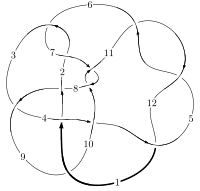
\includegraphics[width=112pt]{../../../GIT/diagram.site/Diagrams/png/1856_12a_1055.png}\\
\ \ \ A knot diagram\footnotemark}&
\allowdisplaybreaks
\textbf{Linearized knot diagam} \\
\cline{2-2}
 &
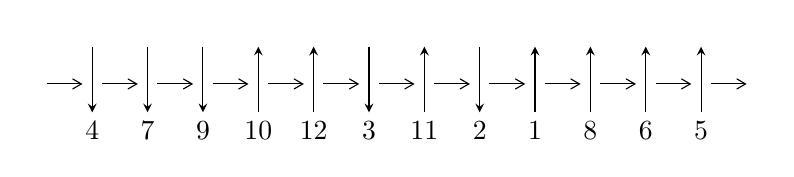
\begin{tikzpicture}[x=20pt, y=17pt]
	% nodes
	\node (C0) at (0, 0) {};
	\node (C1) at (1, 0) {};
	\node (C1U) at (1, +1) {};
	\node (C1D) at (1, -1) {4};

	\node (C2) at (2, 0) {};
	\node (C2U) at (2, +1) {};
	\node (C2D) at (2, -1) {7};

	\node (C3) at (3, 0) {};
	\node (C3U) at (3, +1) {};
	\node (C3D) at (3, -1) {9};

	\node (C4) at (4, 0) {};
	\node (C4U) at (4, +1) {};
	\node (C4D) at (4, -1) {10};

	\node (C5) at (5, 0) {};
	\node (C5U) at (5, +1) {};
	\node (C5D) at (5, -1) {12};

	\node (C6) at (6, 0) {};
	\node (C6U) at (6, +1) {};
	\node (C6D) at (6, -1) {3};

	\node (C7) at (7, 0) {};
	\node (C7U) at (7, +1) {};
	\node (C7D) at (7, -1) {11};

	\node (C8) at (8, 0) {};
	\node (C8U) at (8, +1) {};
	\node (C8D) at (8, -1) {2};

	\node (C9) at (9, 0) {};
	\node (C9U) at (9, +1) {};
	\node (C9D) at (9, -1) {1};

	\node (C10) at (10, 0) {};
	\node (C10U) at (10, +1) {};
	\node (C10D) at (10, -1) {8};

	\node (C11) at (11, 0) {};
	\node (C11U) at (11, +1) {};
	\node (C11D) at (11, -1) {6};

	\node (C12) at (12, 0) {};
	\node (C12U) at (12, +1) {};
	\node (C12D) at (12, -1) {5};
	\node (C13) at (13, 0) {};

	% arrows
	\draw[->,>={angle 60}]
	(C0) edge (C1) (C1) edge (C2) (C2) edge (C3) (C3) edge (C4) (C4) edge (C5) (C5) edge (C6) (C6) edge (C7) (C7) edge (C8) (C8) edge (C9) (C9) edge (C10) (C10) edge (C11) (C11) edge (C12) (C12) edge (C13) ;	\draw[->,>=stealth]
	(C1U) edge (C1D) (C2U) edge (C2D) (C3U) edge (C3D) (C4D) edge (C4U) (C5D) edge (C5U) (C6U) edge (C6D) (C7D) edge (C7U) (C8U) edge (C8D) (C9D) edge (C9U) (C10D) edge (C10U) (C11D) edge (C11U) (C12D) edge (C12U) ;
	\end{tikzpicture} \\
\hhline{~~} \\& 
\textbf{Solving Sequence} \\ \cline{2-2} 
 &
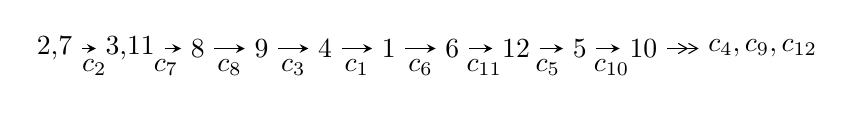
\begin{tikzpicture}[x=23pt, y=7pt]
	% node
	\node (A0) at (-1/8, 0) {2,7};
	\node (A1) at (17/16, 0) {3,11};
	\node (A2) at (17/8, 0) {8};
	\node (A3) at (25/8, 0) {9};
	\node (A4) at (33/8, 0) {4};
	\node (A5) at (41/8, 0) {1};
	\node (A6) at (49/8, 0) {6};
	\node (A7) at (57/8, 0) {12};
	\node (A8) at (65/8, 0) {5};
	\node (A9) at (73/8, 0) {10};
	\node (C1) at (1/2, -1) {$c_{2}$};
	\node (C2) at (13/8, -1) {$c_{7}$};
	\node (C3) at (21/8, -1) {$c_{8}$};
	\node (C4) at (29/8, -1) {$c_{3}$};
	\node (C5) at (37/8, -1) {$c_{1}$};
	\node (C6) at (45/8, -1) {$c_{6}$};
	\node (C7) at (53/8, -1) {$c_{11}$};
	\node (C8) at (61/8, -1) {$c_{5}$};
	\node (C9) at (69/8, -1) {$c_{10}$};
	\node (A10) at (11, 0) {$c_{4},c_{9},c_{12}$};

	% edge
	\draw[->,>=stealth]	
	(A0) edge (A1) (A1) edge (A2) (A2) edge (A3) (A3) edge (A4) (A4) edge (A5) (A5) edge (A6) (A6) edge (A7) (A7) edge (A8) (A8) edge (A9) ;
	\draw[->>,>={angle 60}]	
	(A9) edge (A10);
\end{tikzpicture} \\ 

\end{tabular} \\

\footnotetext{
The image of knot diagram is generated by the software ``\textbf{Draw programme}" developed by Andrew Bartholomew(\url{http://www.layer8.co.uk/maths/draw/index.htm\#Running-draw}), where we modified some parts for our purpose(\url{https://github.com/CATsTAILs/LinksPainter}).
}\phantom \\ \newline 
\centering \textbf{Ideals for irreducible components\footnotemark of $X_{\text{par}}$} 
 
\begin{align*}
I^u_{1}&=\langle 
-2.17270\times10^{674} u^{143}+1.84276\times10^{675} u^{142}+\cdots+2.58449\times10^{677} b+5.69888\times10^{678},\\
\phantom{I^u_{1}}&\phantom{= \langle  }5.38072\times10^{678} u^{143}+8.23180\times10^{678} u^{142}+\cdots+2.55606\times10^{680} a-2.46598\times10^{681},\\
\phantom{I^u_{1}}&\phantom{= \langle  }u^{144}+u^{143}+\cdots-5896 u+989\rangle \\
I^u_{2}&=\langle 
2.35537\times10^{30} u^{39}+1.05919\times10^{30} u^{38}+\cdots+2.44460\times10^{29} b-7.09475\times10^{30},\\
\phantom{I^u_{2}}&\phantom{= \langle  }-7.27177\times10^{30} u^{39}-1.23813\times10^{31} u^{38}+\cdots+2.44460\times10^{29} a+2.34572\times10^{30},\;u^{40}+2 u^{39}+\cdots+2 u+1\rangle \\
\\
\end{align*}
\raggedright * 2 irreducible components of $\dim_{\mathbb{C}}=0$, with total 184 representations.\\
\footnotetext{All coefficients of polynomials are rational numbers. But the coefficients are sometimes approximated in decimal forms when there is not enough margin.}
\newpage
\renewcommand{\arraystretch}{1}
\centering \section*{I. $I^u_{1}= \langle -2.17\times10^{674} u^{143}+1.84\times10^{675} u^{142}+\cdots+2.58\times10^{677} b+5.70\times10^{678},\;5.38\times10^{678} u^{143}+8.23\times10^{678} u^{142}+\cdots+2.56\times10^{680} a-2.47\times10^{681},\;u^{144}+u^{143}+\cdots-5896 u+989 \rangle$}
\flushleft \textbf{(i) Arc colorings}\\
\begin{tabular}{m{7pt} m{180pt} m{7pt} m{180pt} }
\flushright $a_{2}=$&$\begin{pmatrix}1\\0\end{pmatrix}$ \\
\flushright $a_{7}=$&$\begin{pmatrix}0\\u\end{pmatrix}$ \\
\flushright $a_{3}=$&$\begin{pmatrix}1\\u^2\end{pmatrix}$ \\
\flushright $a_{11}=$&$\begin{pmatrix}-0.0210508 u^{143}-0.0322050 u^{142}+\cdots-109.801 u+9.64757\\0.000840669 u^{143}-0.00713005 u^{142}+\cdots+103.422 u-22.0503\end{pmatrix}$ \\
\flushright $a_{8}=$&$\begin{pmatrix}0.0253537 u^{143}+0.0104650 u^{142}+\cdots+455.891 u-94.6977\\0.00283709 u^{143}+0.00148924 u^{142}+\cdots+18.9687 u-4.22269\end{pmatrix}$ \\
\flushright $a_{9}=$&$\begin{pmatrix}0.0225166 u^{143}+0.00897573 u^{142}+\cdots+436.922 u-90.4750\\0.00283709 u^{143}+0.00148924 u^{142}+\cdots+18.9687 u-4.22269\end{pmatrix}$ \\
\flushright $a_{4}=$&$\begin{pmatrix}-0.0196348 u^{143}-0.0664906 u^{142}+\cdots+301.113 u-86.8414\\-0.0258564 u^{143}-0.0394073 u^{142}+\cdots-111.551 u+11.5497\end{pmatrix}$ \\
\flushright $a_{1}=$&$\begin{pmatrix}-0.0676036 u^{143}-0.105365 u^{142}+\cdots-317.722 u+28.5588\\-0.00635388 u^{143}+0.00430054 u^{142}+\cdots-146.861 u+30.0276\end{pmatrix}$ \\
\flushright $a_{6}=$&$\begin{pmatrix}u\\u^3+u\end{pmatrix}$ \\
\flushright $a_{12}=$&$\begin{pmatrix}-0.0281418 u^{143}-0.0439491 u^{142}+\cdots-131.963 u+9.36949\\-0.00598204 u^{143}-0.0163303 u^{142}+\cdots+60.8374 u-17.7264\end{pmatrix}$ \\
\flushright $a_{5}=$&$\begin{pmatrix}-0.0195811 u^{143}+0.00160936 u^{142}+\cdots-476.589 u+101.810\\-0.000614508 u^{143}+0.000419443 u^{142}+\cdots-14.7609 u+5.86952\end{pmatrix}$ \\
\flushright $a_{10}=$&$\begin{pmatrix}0.0796632 u^{143}+0.130380 u^{142}+\cdots+238.971 u-3.85049\\0.0103227 u^{143}+0.00404013 u^{142}+\cdots+172.885 u-34.7918\end{pmatrix}$\\&\end{tabular}
\flushleft \textbf{(ii) Obstruction class $= -1$}\\~\\
\flushleft \textbf{(iii) Cusp Shapes $= 0.0628033 u^{143}+0.00950011 u^{142}+\cdots+1209.64 u-250.992$}\\~\\
\newpage\renewcommand{\arraystretch}{1}
\flushleft \textbf{(iv) u-Polynomials at the component}\newline \\
\begin{tabular}{m{50pt}|m{274pt}}
Crossings & \hspace{64pt}u-Polynomials at each crossing \\
\hline $$\begin{aligned}c_{1}\end{aligned}$$&$\begin{aligned}
&u^{144}-5 u^{143}+\cdots-106 u+17
\end{aligned}$\\
\hline $$\begin{aligned}c_{2},c_{6}\end{aligned}$$&$\begin{aligned}
&u^{144}- u^{143}+\cdots+5896 u+989
\end{aligned}$\\
\hline $$\begin{aligned}c_{3}\end{aligned}$$&$\begin{aligned}
&u^{144}+u^{143}+\cdots-431616 u+85504
\end{aligned}$\\
\hline $$\begin{aligned}c_{4}\end{aligned}$$&$\begin{aligned}
&u^{144}- u^{143}+\cdots+545 u+307
\end{aligned}$\\
\hline $$\begin{aligned}c_{5},c_{11},c_{12}\end{aligned}$$&$\begin{aligned}
&u^{144}- u^{143}+\cdots+2435 u+193
\end{aligned}$\\
\hline $$\begin{aligned}c_{7},c_{10}\end{aligned}$$&$\begin{aligned}
&u^{144}-7 u^{143}+\cdots+126358 u+11033
\end{aligned}$\\
\hline $$\begin{aligned}c_{8}\end{aligned}$$&$\begin{aligned}
&u^{144}+u^{143}+\cdots+222158 u+28393
\end{aligned}$\\
\hline $$\begin{aligned}c_{9}\end{aligned}$$&$\begin{aligned}
&u^{144}-3 u^{143}+\cdots-94488 u+22681
\end{aligned}$\\
\hline
\end{tabular}\\~\\
\newpage\renewcommand{\arraystretch}{1}
\flushleft \textbf{(v) Riley Polynomials at the component}\newline \\
\begin{tabular}{m{50pt}|m{274pt}}
Crossings & \hspace{64pt}Riley Polynomials at each crossing \\
\hline $$\begin{aligned}c_{1}\end{aligned}$$&$\begin{aligned}
&y^{144}+17 y^{143}+\cdots+8926 y+289
\end{aligned}$\\
\hline $$\begin{aligned}c_{2},c_{6}\end{aligned}$$&$\begin{aligned}
&y^{144}+65 y^{143}+\cdots+23149068 y+978121
\end{aligned}$\\
\hline $$\begin{aligned}c_{3}\end{aligned}$$&$\begin{aligned}
&y^{144}-5 y^{143}+\cdots-279517724672 y+7310934016
\end{aligned}$\\
\hline $$\begin{aligned}c_{4}\end{aligned}$$&$\begin{aligned}
&y^{144}+51 y^{143}+\cdots+4212805 y+94249
\end{aligned}$\\
\hline $$\begin{aligned}c_{5},c_{11},c_{12}\end{aligned}$$&$\begin{aligned}
&y^{144}+161 y^{143}+\cdots+3654383 y+37249
\end{aligned}$\\
\hline $$\begin{aligned}c_{7},c_{10}\end{aligned}$$&$\begin{aligned}
&y^{144}+87 y^{143}+\cdots+4474494936 y+121727089
\end{aligned}$\\
\hline $$\begin{aligned}c_{8}\end{aligned}$$&$\begin{aligned}
&y^{144}+25 y^{143}+\cdots+51876294512 y+806162449
\end{aligned}$\\
\hline $$\begin{aligned}c_{9}\end{aligned}$$&$\begin{aligned}
&y^{144}+37 y^{143}+\cdots+31337234260 y+514427761
\end{aligned}$\\
\hline
\end{tabular}\\~\\
\newpage\flushleft \textbf{(vi) Complex Volumes and Cusp Shapes}
$$\begin{array}{c|c|c}  
\text{Solutions to }I^u_{1}& \I (\text{vol} + \sqrt{-1}CS) & \text{Cusp shape}\\
 \hline 
\begin{aligned}
u &= \phantom{-}0.517855 + 0.858761 I \\
a &= \phantom{-}1.07131 - 1.17568 I \\
b &= \phantom{-}0.422535 - 0.489625 I\end{aligned}
 & -1.32577 - 2.09615 I & \phantom{-0.000000 } 0 \\ \hline\begin{aligned}
u &= \phantom{-}0.517855 - 0.858761 I \\
a &= \phantom{-}1.07131 + 1.17568 I \\
b &= \phantom{-}0.422535 + 0.489625 I\end{aligned}
 & -1.32577 + 2.09615 I & \phantom{-0.000000 } 0 \\ \hline\begin{aligned}
u &= -0.355540 + 0.926995 I \\
a &= -0.92831 - 1.29737 I \\
b &= \phantom{-}0.284858 - 0.363499 I\end{aligned}
 & -2.00130 + 1.43707 I & \phantom{-0.000000 } 0 \\ \hline\begin{aligned}
u &= -0.355540 - 0.926995 I \\
a &= -0.92831 + 1.29737 I \\
b &= \phantom{-}0.284858 + 0.363499 I\end{aligned}
 & -2.00130 - 1.43707 I & \phantom{-0.000000 } 0 \\ \hline\begin{aligned}
u &= -0.228469 + 0.962555 I \\
a &= -0.523580 - 1.184250 I \\
b &= -0.509620 - 0.276973 I\end{aligned}
 & \phantom{-}4.12127 + 0.74656 I & \phantom{-0.000000 } 0 \\ \hline\begin{aligned}
u &= -0.228469 - 0.962555 I \\
a &= -0.523580 + 1.184250 I \\
b &= -0.509620 + 0.276973 I\end{aligned}
 & \phantom{-}4.12127 - 0.74656 I & \phantom{-0.000000 } 0 \\ \hline\begin{aligned}
u &= \phantom{-}0.063001 + 1.022290 I \\
a &= \phantom{-}0.375022 - 1.209370 I \\
b &= -0.184033 - 0.290733 I\end{aligned}
 & \phantom{-}4.32694 + 0.06920 I & \phantom{-0.000000 } 0 \\ \hline\begin{aligned}
u &= \phantom{-}0.063001 - 1.022290 I \\
a &= \phantom{-}0.375022 + 1.209370 I \\
b &= -0.184033 + 0.290733 I\end{aligned}
 & \phantom{-}4.32694 - 0.06920 I & \phantom{-0.000000 } 0 \\ \hline\begin{aligned}
u &= -0.424519 + 0.872191 I \\
a &= \phantom{-}0.956076 - 0.683640 I \\
b &= -0.09268 - 2.12496 I\end{aligned}
 & -3.24788 + 4.70970 I & \phantom{-0.000000 } 0 \\ \hline\begin{aligned}
u &= -0.424519 - 0.872191 I \\
a &= \phantom{-}0.956076 + 0.683640 I \\
b &= -0.09268 + 2.12496 I\end{aligned}
 & -3.24788 - 4.70970 I & \phantom{-0.000000 } 0\\
 \hline 
 \end{array}$$\newpage$$\begin{array}{c|c|c}  
\text{Solutions to }I^u_{1}& \I (\text{vol} + \sqrt{-1}CS) & \text{Cusp shape}\\
 \hline 
\begin{aligned}
u &= -0.427690 + 0.843847 I \\
a &= -1.149220 + 0.698741 I \\
b &= \phantom{-}1.25378 + 1.49091 I\end{aligned}
 & -3.33926 - 1.12138 I & \phantom{-0.000000 } 0 \\ \hline\begin{aligned}
u &= -0.427690 - 0.843847 I \\
a &= -1.149220 - 0.698741 I \\
b &= \phantom{-}1.25378 - 1.49091 I\end{aligned}
 & -3.33926 + 1.12138 I & \phantom{-0.000000 } 0 \\ \hline\begin{aligned}
u &= -1.013940 + 0.328197 I \\
a &= \phantom{-}0.700021 - 0.866564 I \\
b &= -0.01062 - 1.73100 I\end{aligned}
 & -3.04638 - 8.74887 I & \phantom{-0.000000 } 0 \\ \hline\begin{aligned}
u &= -1.013940 - 0.328197 I \\
a &= \phantom{-}0.700021 + 0.866564 I \\
b &= -0.01062 + 1.73100 I\end{aligned}
 & -3.04638 + 8.74887 I & \phantom{-0.000000 } 0 \\ \hline\begin{aligned}
u &= \phantom{-}1.027860 + 0.283936 I \\
a &= -0.400907 - 0.889539 I \\
b &= \phantom{-}0.36679 - 1.72986 I\end{aligned}
 & -4.61579 + 0.14727 I & \phantom{-0.000000 } 0 \\ \hline\begin{aligned}
u &= \phantom{-}1.027860 - 0.283936 I \\
a &= -0.400907 + 0.889539 I \\
b &= \phantom{-}0.36679 + 1.72986 I\end{aligned}
 & -4.61579 - 0.14727 I & \phantom{-0.000000 } 0 \\ \hline\begin{aligned}
u &= -0.442077 + 0.972988 I \\
a &= \phantom{-}1.158990 - 0.636061 I \\
b &= -1.026780 - 0.947011 I\end{aligned}
 & -2.97543 + 5.01417 I & \phantom{-0.000000 } 0 \\ \hline\begin{aligned}
u &= -0.442077 - 0.972988 I \\
a &= \phantom{-}1.158990 + 0.636061 I \\
b &= -1.026780 + 0.947011 I\end{aligned}
 & -2.97543 - 5.01417 I & \phantom{-0.000000 } 0 \\ \hline\begin{aligned}
u &= \phantom{-}1.000520 + 0.384416 I \\
a &= \phantom{-}0.84725 + 1.13480 I \\
b &= \phantom{-}0.11867 + 1.47304 I\end{aligned}
 & -7.85810 + 4.18783 I & \phantom{-0.000000 } 0 \\ \hline\begin{aligned}
u &= \phantom{-}1.000520 - 0.384416 I \\
a &= \phantom{-}0.84725 - 1.13480 I \\
b &= \phantom{-}0.11867 - 1.47304 I\end{aligned}
 & -7.85810 - 4.18783 I & \phantom{-0.000000 } 0\\
 \hline 
 \end{array}$$\newpage$$\begin{array}{c|c|c}  
\text{Solutions to }I^u_{1}& \I (\text{vol} + \sqrt{-1}CS) & \text{Cusp shape}\\
 \hline 
\begin{aligned}
u &= -0.633669 + 0.876521 I \\
a &= \phantom{-}0.299556 - 0.921499 I \\
b &= -1.00999 - 1.36150 I\end{aligned}
 & \phantom{-}1.75567 + 4.34220 I & \phantom{-0.000000 } 0 \\ \hline\begin{aligned}
u &= -0.633669 - 0.876521 I \\
a &= \phantom{-}0.299556 + 0.921499 I \\
b &= -1.00999 + 1.36150 I\end{aligned}
 & \phantom{-}1.75567 - 4.34220 I & \phantom{-0.000000 } 0 \\ \hline\begin{aligned}
u &= -0.708842 + 0.572621 I \\
a &= \phantom{-}1.30572 - 0.88155 I \\
b &= -0.339536 - 0.635963 I\end{aligned}
 & -10.40510 + 0.69580 I & \phantom{-0.000000 } 0 \\ \hline\begin{aligned}
u &= -0.708842 - 0.572621 I \\
a &= \phantom{-}1.30572 + 0.88155 I \\
b &= -0.339536 + 0.635963 I\end{aligned}
 & -10.40510 - 0.69580 I & \phantom{-0.000000 } 0 \\ \hline\begin{aligned}
u &= \phantom{-}0.610838 + 0.902898 I \\
a &= \phantom{-}0.715158 + 0.400766 I \\
b &= \phantom{-}0.03549 + 1.68791 I\end{aligned}
 & -0.92355 - 1.16423 I & \phantom{-0.000000 } 0 \\ \hline\begin{aligned}
u &= \phantom{-}0.610838 - 0.902898 I \\
a &= \phantom{-}0.715158 - 0.400766 I \\
b &= \phantom{-}0.03549 - 1.68791 I\end{aligned}
 & -0.92355 + 1.16423 I & \phantom{-0.000000 } 0 \\ \hline\begin{aligned}
u &= \phantom{-}0.560258 + 0.696446 I \\
a &= -0.570660 - 0.624073 I \\
b &= \phantom{-}1.002330 - 0.488793 I\end{aligned}
 & -0.96818 - 1.42189 I & \phantom{-0.000000 } 0 \\ \hline\begin{aligned}
u &= \phantom{-}0.560258 - 0.696446 I \\
a &= -0.570660 + 0.624073 I \\
b &= \phantom{-}1.002330 + 0.488793 I\end{aligned}
 & -0.96818 + 1.42189 I & \phantom{-0.000000 } 0 \\ \hline\begin{aligned}
u &= -0.303732 + 1.066140 I \\
a &= -0.733376 - 0.446451 I \\
b &= -0.088832 + 0.426032 I\end{aligned}
 & \phantom{-}2.36848 - 0.79913 I & \phantom{-0.000000 } 0 \\ \hline\begin{aligned}
u &= -0.303732 - 1.066140 I \\
a &= -0.733376 + 0.446451 I \\
b &= -0.088832 - 0.426032 I\end{aligned}
 & \phantom{-}2.36848 + 0.79913 I & \phantom{-0.000000 } 0\\
 \hline 
 \end{array}$$\newpage$$\begin{array}{c|c|c}  
\text{Solutions to }I^u_{1}& \I (\text{vol} + \sqrt{-1}CS) & \text{Cusp shape}\\
 \hline 
\begin{aligned}
u &= \phantom{-}0.266885 + 1.078750 I \\
a &= -0.276052 + 0.400419 I \\
b &= \phantom{-}0.076490 + 0.488818 I\end{aligned}
 & \phantom{-}1.10377 - 2.05634 I & \phantom{-0.000000 } 0 \\ \hline\begin{aligned}
u &= \phantom{-}0.266885 - 1.078750 I \\
a &= -0.276052 - 0.400419 I \\
b &= \phantom{-}0.076490 - 0.488818 I\end{aligned}
 & \phantom{-}1.10377 + 2.05634 I & \phantom{-0.000000 } 0 \\ \hline\begin{aligned}
u &= -0.456686 + 0.759218 I \\
a &= -0.931926 + 1.023090 I \\
b &= -0.14489 + 1.45922 I\end{aligned}
 & -3.62940 - 1.30889 I & \phantom{-0.000000 } 0 \\ \hline\begin{aligned}
u &= -0.456686 - 0.759218 I \\
a &= -0.931926 - 1.023090 I \\
b &= -0.14489 - 1.45922 I\end{aligned}
 & -3.62940 + 1.30889 I & \phantom{-0.000000 } 0 \\ \hline\begin{aligned}
u &= \phantom{-}0.125732 + 1.107930 I \\
a &= \phantom{-}0.837788 + 0.386447 I \\
b &= -1.47232 + 0.33107 I\end{aligned}
 & -1.85603 + 5.07461 I & \phantom{-0.000000 } 0 \\ \hline\begin{aligned}
u &= \phantom{-}0.125732 - 1.107930 I \\
a &= \phantom{-}0.837788 - 0.386447 I \\
b &= -1.47232 - 0.33107 I\end{aligned}
 & -1.85603 - 5.07461 I & \phantom{-0.000000 } 0 \\ \hline\begin{aligned}
u &= \phantom{-}0.494450 + 0.726951 I \\
a &= -0.85345 - 1.22710 I \\
b &= \phantom{-}1.39694 - 1.24451 I\end{aligned}
 & -1.60214 - 3.42664 I & \phantom{-0.000000 } 0 \\ \hline\begin{aligned}
u &= \phantom{-}0.494450 - 0.726951 I \\
a &= -0.85345 + 1.22710 I \\
b &= \phantom{-}1.39694 + 1.24451 I\end{aligned}
 & -1.60214 + 3.42664 I & \phantom{-0.000000 } 0 \\ \hline\begin{aligned}
u &= \phantom{-}0.127020 + 1.114490 I \\
a &= \phantom{-}0.455851 - 0.633263 I \\
b &= \phantom{-}1.097710 + 0.273582 I\end{aligned}
 & \phantom{-}1.16957 + 1.11750 I & \phantom{-0.000000 } 0 \\ \hline\begin{aligned}
u &= \phantom{-}0.127020 - 1.114490 I \\
a &= \phantom{-}0.455851 + 0.633263 I \\
b &= \phantom{-}1.097710 - 0.273582 I\end{aligned}
 & \phantom{-}1.16957 - 1.11750 I & \phantom{-0.000000 } 0\\
 \hline 
 \end{array}$$\newpage$$\begin{array}{c|c|c}  
\text{Solutions to }I^u_{1}& \I (\text{vol} + \sqrt{-1}CS) & \text{Cusp shape}\\
 \hline 
\begin{aligned}
u &= \phantom{-}0.168145 + 1.127140 I \\
a &= -0.158159 - 0.844049 I \\
b &= -0.125944 - 0.188979 I\end{aligned}
 & \phantom{-}3.53079 - 2.66328 I & \phantom{-0.000000 } 0 \\ \hline\begin{aligned}
u &= \phantom{-}0.168145 - 1.127140 I \\
a &= -0.158159 + 0.844049 I \\
b &= -0.125944 + 0.188979 I\end{aligned}
 & \phantom{-}3.53079 + 2.66328 I & \phantom{-0.000000 } 0 \\ \hline\begin{aligned}
u &= \phantom{-}0.700144 + 0.900884 I \\
a &= \phantom{-}1.145280 - 0.297858 I \\
b &= \phantom{-}0.146788 + 0.452565 I\end{aligned}
 & -3.29013 + 0.66050 I & \phantom{-0.000000 } 0 \\ \hline\begin{aligned}
u &= \phantom{-}0.700144 - 0.900884 I \\
a &= \phantom{-}1.145280 + 0.297858 I \\
b &= \phantom{-}0.146788 - 0.452565 I\end{aligned}
 & -3.29013 - 0.66050 I & \phantom{-0.000000 } 0 \\ \hline\begin{aligned}
u &= -0.390874 + 1.081960 I \\
a &= \phantom{-}0.750270 - 0.412185 I \\
b &= \phantom{-}0.96387 - 1.56771 I\end{aligned}
 & -6.93969 + 2.57610 I & \phantom{-0.000000 } 0 \\ \hline\begin{aligned}
u &= -0.390874 - 1.081960 I \\
a &= \phantom{-}0.750270 + 0.412185 I \\
b &= \phantom{-}0.96387 + 1.56771 I\end{aligned}
 & -6.93969 - 2.57610 I & \phantom{-0.000000 } 0 \\ \hline\begin{aligned}
u &= \phantom{-}0.482016 + 1.049150 I \\
a &= \phantom{-}0.858899 + 0.746632 I \\
b &= -1.51305 + 1.73571 I\end{aligned}
 & \phantom{-}0.24985 - 7.82066 I & \phantom{-0.000000 } 0 \\ \hline\begin{aligned}
u &= \phantom{-}0.482016 - 1.049150 I \\
a &= \phantom{-}0.858899 - 0.746632 I \\
b &= -1.51305 - 1.73571 I\end{aligned}
 & \phantom{-}0.24985 + 7.82066 I & \phantom{-0.000000 } 0 \\ \hline\begin{aligned}
u &= -1.131750 + 0.241574 I \\
a &= \phantom{-}0.100307 - 1.130640 I \\
b &= -0.678773 - 1.219620 I\end{aligned}
 & -10.25730 + 3.14256 I & \phantom{-0.000000 } 0 \\ \hline\begin{aligned}
u &= -1.131750 - 0.241574 I \\
a &= \phantom{-}0.100307 + 1.130640 I \\
b &= -0.678773 + 1.219620 I\end{aligned}
 & -10.25730 - 3.14256 I & \phantom{-0.000000 } 0\\
 \hline 
 \end{array}$$\newpage$$\begin{array}{c|c|c}  
\text{Solutions to }I^u_{1}& \I (\text{vol} + \sqrt{-1}CS) & \text{Cusp shape}\\
 \hline 
\begin{aligned}
u &= -0.214027 + 0.813486 I \\
a &= \phantom{-}1.10150 - 1.09864 I \\
b &= -0.814823 - 1.152660 I\end{aligned}
 & \phantom{-}1.16885 + 3.08474 I & \phantom{-0.000000 } 0 \\ \hline\begin{aligned}
u &= -0.214027 - 0.813486 I \\
a &= \phantom{-}1.10150 + 1.09864 I \\
b &= -0.814823 + 1.152660 I\end{aligned}
 & \phantom{-}1.16885 - 3.08474 I & \phantom{-0.000000 } 0 \\ \hline\begin{aligned}
u &= -0.649790 + 0.510668 I \\
a &= \phantom{-}0.773497 + 0.135585 I \\
b &= -0.186296 + 0.931616 I\end{aligned}
 & -7.21083 - 0.39117 I & \phantom{-0.000000 } 0 \\ \hline\begin{aligned}
u &= -0.649790 - 0.510668 I \\
a &= \phantom{-}0.773497 - 0.135585 I \\
b &= -0.186296 - 0.931616 I\end{aligned}
 & -7.21083 + 0.39117 I & \phantom{-0.000000 } 0 \\ \hline\begin{aligned}
u &= -0.579659 + 1.036620 I \\
a &= \phantom{-}0.742083 - 1.006530 I \\
b &= -1.06629 - 1.75122 I\end{aligned}
 & \phantom{-}0.33040 + 7.23718 I & \phantom{-0.000000 } 0 \\ \hline\begin{aligned}
u &= -0.579659 - 1.036620 I \\
a &= \phantom{-}0.742083 + 1.006530 I \\
b &= -1.06629 + 1.75122 I\end{aligned}
 & \phantom{-}0.33040 - 7.23718 I & \phantom{-0.000000 } 0 \\ \hline\begin{aligned}
u &= -0.608949 + 1.025090 I \\
a &= \phantom{-}0.555994 + 0.603439 I \\
b &= -0.091363 + 0.327585 I\end{aligned}
 & -5.72956 + 5.36982 I & \phantom{-0.000000 } 0 \\ \hline\begin{aligned}
u &= -0.608949 - 1.025090 I \\
a &= \phantom{-}0.555994 - 0.603439 I \\
b &= -0.091363 - 0.327585 I\end{aligned}
 & -5.72956 - 5.36982 I & \phantom{-0.000000 } 0 \\ \hline\begin{aligned}
u &= -0.436203 + 1.112580 I \\
a &= -0.541794 + 0.639987 I \\
b &= \phantom{-}1.04481 + 1.09676 I\end{aligned}
 & \phantom{-}2.76565 - 0.81161 I & \phantom{-0.000000 } 0 \\ \hline\begin{aligned}
u &= -0.436203 - 1.112580 I \\
a &= -0.541794 - 0.639987 I \\
b &= \phantom{-}1.04481 - 1.09676 I\end{aligned}
 & \phantom{-}2.76565 + 0.81161 I & \phantom{-0.000000 } 0\\
 \hline 
 \end{array}$$\newpage$$\begin{array}{c|c|c}  
\text{Solutions to }I^u_{1}& \I (\text{vol} + \sqrt{-1}CS) & \text{Cusp shape}\\
 \hline 
\begin{aligned}
u &= -0.613093 + 0.516769 I \\
a &= -1.17848 + 0.78233 I \\
b &= \phantom{-}0.04086 + 1.47264 I\end{aligned}
 & -1.18560 - 2.48718 I & \phantom{-0.000000 } 0 \\ \hline\begin{aligned}
u &= -0.613093 - 0.516769 I \\
a &= -1.17848 - 0.78233 I \\
b &= \phantom{-}0.04086 - 1.47264 I\end{aligned}
 & -1.18560 + 2.48718 I & \phantom{-0.000000 } 0 \\ \hline\begin{aligned}
u &= \phantom{-}0.575581 + 1.054390 I \\
a &= -0.750827 + 0.918826 I \\
b &= -0.207997 + 0.084971 I\end{aligned}
 & -4.32792 - 12.04850 I & \phantom{-0.000000 } 0 \\ \hline\begin{aligned}
u &= \phantom{-}0.575581 - 1.054390 I \\
a &= -0.750827 - 0.918826 I \\
b &= -0.207997 - 0.084971 I\end{aligned}
 & -4.32792 + 12.04850 I & \phantom{-0.000000 } 0 \\ \hline\begin{aligned}
u &= \phantom{-}0.814552 + 0.918703 I \\
a &= \phantom{-}0.010307 - 1.024020 I \\
b &= \phantom{-}0.74676 - 1.67595 I\end{aligned}
 & -3.37246 - 6.44630 I & \phantom{-0.000000 } 0 \\ \hline\begin{aligned}
u &= \phantom{-}0.814552 - 0.918703 I \\
a &= \phantom{-}0.010307 + 1.024020 I \\
b &= \phantom{-}0.74676 + 1.67595 I\end{aligned}
 & -3.37246 + 6.44630 I & \phantom{-0.000000 } 0 \\ \hline\begin{aligned}
u &= \phantom{-}0.573243 + 0.511294 I \\
a &= -1.154820 + 0.608881 I \\
b &= -0.199791 + 1.255340 I\end{aligned}
 & -5.97031 + 7.35454 I & \phantom{-0.000000 } 0 \\ \hline\begin{aligned}
u &= \phantom{-}0.573243 - 0.511294 I \\
a &= -1.154820 - 0.608881 I \\
b &= -0.199791 - 1.255340 I\end{aligned}
 & -5.97031 - 7.35454 I & \phantom{-0.000000 } 0 \\ \hline\begin{aligned}
u &= \phantom{-}0.448637 + 1.149920 I \\
a &= -0.735635 - 0.876913 I \\
b &= \phantom{-}0.75668 - 1.20545 I\end{aligned}
 & \phantom{-}1.30780 - 6.55447 I & \phantom{-0.000000 } 0 \\ \hline\begin{aligned}
u &= \phantom{-}0.448637 - 1.149920 I \\
a &= -0.735635 + 0.876913 I \\
b &= \phantom{-}0.75668 + 1.20545 I\end{aligned}
 & \phantom{-}1.30780 + 6.55447 I & \phantom{-0.000000 } 0\\
 \hline 
 \end{array}$$\newpage$$\begin{array}{c|c|c}  
\text{Solutions to }I^u_{1}& \I (\text{vol} + \sqrt{-1}CS) & \text{Cusp shape}\\
 \hline 
\begin{aligned}
u &= \phantom{-}0.505675 + 1.126910 I \\
a &= \phantom{-}0.854993 + 0.881546 I \\
b &= \phantom{-}0.07486 + 1.46044 I\end{aligned}
 & -9.64904 + 1.20544 I & \phantom{-0.000000 } 0 \\ \hline\begin{aligned}
u &= \phantom{-}0.505675 - 1.126910 I \\
a &= \phantom{-}0.854993 - 0.881546 I \\
b &= \phantom{-}0.07486 - 1.46044 I\end{aligned}
 & -9.64904 - 1.20544 I & \phantom{-0.000000 } 0 \\ \hline\begin{aligned}
u &= -0.625956 + 1.065260 I \\
a &= -0.464025 + 0.929483 I \\
b &= \phantom{-}0.04685 + 1.50346 I\end{aligned}
 & -8.88424 + 4.46607 I & \phantom{-0.000000 } 0 \\ \hline\begin{aligned}
u &= -0.625956 - 1.065260 I \\
a &= -0.464025 - 0.929483 I \\
b &= \phantom{-}0.04685 - 1.50346 I\end{aligned}
 & -8.88424 - 4.46607 I & \phantom{-0.000000 } 0 \\ \hline\begin{aligned}
u &= \phantom{-}0.415061 + 1.164620 I \\
a &= -0.808416 + 0.297906 I \\
b &= \phantom{-}0.578523 - 0.123155 I\end{aligned}
 & \phantom{-}0.541665 + 0.674438 I & \phantom{-0.000000 } 0 \\ \hline\begin{aligned}
u &= \phantom{-}0.415061 - 1.164620 I \\
a &= -0.808416 - 0.297906 I \\
b &= \phantom{-}0.578523 + 0.123155 I\end{aligned}
 & \phantom{-}0.541665 - 0.674438 I & \phantom{-0.000000 } 0 \\ \hline\begin{aligned}
u &= -0.391320 + 1.176750 I \\
a &= \phantom{-}0.419634 + 0.768388 I \\
b &= \phantom{-}0.281154 + 0.101537 I\end{aligned}
 & \phantom{-}3.12719 + 8.75276 I & \phantom{-0.000000 } 0 \\ \hline\begin{aligned}
u &= -0.391320 - 1.176750 I \\
a &= \phantom{-}0.419634 - 0.768388 I \\
b &= \phantom{-}0.281154 - 0.101537 I\end{aligned}
 & \phantom{-}3.12719 - 8.75276 I & \phantom{-0.000000 } 0 \\ \hline\begin{aligned}
u &= \phantom{-}0.529117 + 0.515088 I \\
a &= \phantom{-}0.17738 + 1.41004 I \\
b &= \phantom{-}0.07309 + 1.65251 I\end{aligned}
 & -1.80834 - 4.97274 I & \phantom{-0.000000 } 0 \\ \hline\begin{aligned}
u &= \phantom{-}0.529117 - 0.515088 I \\
a &= \phantom{-}0.17738 - 1.41004 I \\
b &= \phantom{-}0.07309 - 1.65251 I\end{aligned}
 & -1.80834 + 4.97274 I & \phantom{-0.000000 } 0\\
 \hline 
 \end{array}$$\newpage$$\begin{array}{c|c|c}  
\text{Solutions to }I^u_{1}& \I (\text{vol} + \sqrt{-1}CS) & \text{Cusp shape}\\
 \hline 
\begin{aligned}
u &= \phantom{-}0.552350 + 1.142960 I \\
a &= -0.842810 - 0.662161 I \\
b &= -0.16534 - 1.82352 I\end{aligned}
 & -10.03460 - 9.32684 I & \phantom{-0.000000 } 0 \\ \hline\begin{aligned}
u &= \phantom{-}0.552350 - 1.142960 I \\
a &= -0.842810 + 0.662161 I \\
b &= -0.16534 + 1.82352 I\end{aligned}
 & -10.03460 + 9.32684 I & \phantom{-0.000000 } 0 \\ \hline\begin{aligned}
u &= -0.249519 + 0.685647 I \\
a &= -1.81767 + 0.54432 I \\
b &= \phantom{-}1.85314 + 0.14047 I\end{aligned}
 & -8.55206 + 0.30724 I & \phantom{-0.000000 } 0 \\ \hline\begin{aligned}
u &= -0.249519 - 0.685647 I \\
a &= -1.81767 - 0.54432 I \\
b &= \phantom{-}1.85314 - 0.14047 I\end{aligned}
 & -8.55206 - 0.30724 I & \phantom{-0.000000 } 0 \\ \hline\begin{aligned}
u &= -0.544172 + 1.165270 I \\
a &= -0.373268 - 0.595968 I \\
b &= \phantom{-}0.341746 - 0.006999 I\end{aligned}
 & -3.71802 + 3.39018 I & \phantom{-0.000000 } 0 \\ \hline\begin{aligned}
u &= -0.544172 - 1.165270 I \\
a &= -0.373268 + 0.595968 I \\
b &= \phantom{-}0.341746 + 0.006999 I\end{aligned}
 & -3.71802 - 3.39018 I & \phantom{-0.000000 } 0 \\ \hline\begin{aligned}
u &= -1.295510 + 0.079139 I \\
a &= -0.050953 + 0.456006 I \\
b &= -0.18642 + 2.25352 I\end{aligned}
 & -7.70149 - 1.28594 I & \phantom{-0.000000 } 0 \\ \hline\begin{aligned}
u &= -1.295510 - 0.079139 I \\
a &= -0.050953 - 0.456006 I \\
b &= -0.18642 - 2.25352 I\end{aligned}
 & -7.70149 + 1.28594 I & \phantom{-0.000000 } 0 \\ \hline\begin{aligned}
u &= \phantom{-}0.644292 + 0.276965 I \\
a &= -0.625586 - 0.286812 I \\
b &= \phantom{-}0.0650896 - 0.0924493 I\end{aligned}
 & -1.13811 - 1.22929 I & \phantom{-0.000000 } 0 \\ \hline\begin{aligned}
u &= \phantom{-}0.644292 - 0.276965 I \\
a &= -0.625586 + 0.286812 I \\
b &= \phantom{-}0.0650896 + 0.0924493 I\end{aligned}
 & -1.13811 + 1.22929 I & \phantom{-0.000000 } 0\\
 \hline 
 \end{array}$$\newpage$$\begin{array}{c|c|c}  
\text{Solutions to }I^u_{1}& \I (\text{vol} + \sqrt{-1}CS) & \text{Cusp shape}\\
 \hline 
\begin{aligned}
u &= \phantom{-}0.589086 + 1.163640 I \\
a &= \phantom{-}0.679726 + 0.674196 I \\
b &= -0.94054 + 1.88497 I\end{aligned}
 & -1.89596 - 5.69212 I & \phantom{-0.000000 } 0 \\ \hline\begin{aligned}
u &= \phantom{-}0.589086 - 1.163640 I \\
a &= \phantom{-}0.679726 - 0.674196 I \\
b &= -0.94054 - 1.88497 I\end{aligned}
 & -1.89596 + 5.69212 I & \phantom{-0.000000 } 0 \\ \hline\begin{aligned}
u &= \phantom{-}0.416142 + 0.544802 I \\
a &= -0.526173 - 0.598536 I \\
b &= \phantom{-}0.880180 + 0.038644 I\end{aligned}
 & -0.94869 - 1.38584 I & \phantom{-0.000000 -}0. + 4.67960 I \\ \hline\begin{aligned}
u &= \phantom{-}0.416142 - 0.544802 I \\
a &= -0.526173 + 0.598536 I \\
b &= \phantom{-}0.880180 - 0.038644 I\end{aligned}
 & -0.94869 + 1.38584 I & \phantom{-0.000000 } 0. - 4.67960 I \\ \hline\begin{aligned}
u &= \phantom{-}0.564918 + 0.383332 I \\
a &= \phantom{-}1.45545 + 1.93888 I \\
b &= -0.708421 + 1.011680 I\end{aligned}
 & -12.34290 + 4.70339 I & -8.84051 + 0. I\phantom{ +0.000000I} \\ \hline\begin{aligned}
u &= \phantom{-}0.564918 - 0.383332 I \\
a &= \phantom{-}1.45545 - 1.93888 I \\
b &= -0.708421 - 1.011680 I\end{aligned}
 & -12.34290 - 4.70339 I & -8.84051 + 0. I\phantom{ +0.000000I} \\ \hline\begin{aligned}
u &= \phantom{-}1.279420 + 0.322188 I \\
a &= \phantom{-}0.265884 + 0.709923 I \\
b &= \phantom{-}0.05481 + 1.79871 I\end{aligned}
 & -4.14898 + 0.36457 I & \phantom{-0.000000 } 0 \\ \hline\begin{aligned}
u &= \phantom{-}1.279420 - 0.322188 I \\
a &= \phantom{-}0.265884 - 0.709923 I \\
b &= \phantom{-}0.05481 - 1.79871 I\end{aligned}
 & -4.14898 - 0.36457 I & \phantom{-0.000000 } 0 \\ \hline\begin{aligned}
u &= -0.679447 + 0.013049 I \\
a &= \phantom{-}0.864948 - 0.181389 I \\
b &= \phantom{-}0.387957 - 0.800762 I\end{aligned}
 & -0.31375 + 4.79943 I & \phantom{-}1.02873 - 5.75401 I \\ \hline\begin{aligned}
u &= -0.679447 - 0.013049 I \\
a &= \phantom{-}0.864948 + 0.181389 I \\
b &= \phantom{-}0.387957 + 0.800762 I\end{aligned}
 & -0.31375 - 4.79943 I & \phantom{-}1.02873 + 5.75401 I\\
 \hline 
 \end{array}$$\newpage$$\begin{array}{c|c|c}  
\text{Solutions to }I^u_{1}& \I (\text{vol} + \sqrt{-1}CS) & \text{Cusp shape}\\
 \hline 
\begin{aligned}
u &= \phantom{-}0.343291 + 0.582586 I \\
a &= -1.136990 - 0.510742 I \\
b &= -0.05655 - 2.15459 I\end{aligned}
 & -1.38479 + 4.08308 I & \phantom{-0.000000 } 0. - 2.31629 I \\ \hline\begin{aligned}
u &= \phantom{-}0.343291 - 0.582586 I \\
a &= -1.136990 + 0.510742 I \\
b &= -0.05655 + 2.15459 I\end{aligned}
 & -1.38479 - 4.08308 I & \phantom{-0.000000 -}0. + 2.31629 I \\ \hline\begin{aligned}
u &= \phantom{-}0.724269 + 1.110850 I \\
a &= \phantom{-}0.357258 + 0.703821 I \\
b &= -0.60736 + 1.54911 I\end{aligned}
 & \phantom{-}0.27215 - 4.05186 I & \phantom{-0.000000 } 0 \\ \hline\begin{aligned}
u &= \phantom{-}0.724269 - 1.110850 I \\
a &= \phantom{-}0.357258 - 0.703821 I \\
b &= -0.60736 - 1.54911 I\end{aligned}
 & \phantom{-}0.27215 + 4.05186 I & \phantom{-0.000000 } 0 \\ \hline\begin{aligned}
u &= -0.645742 + 1.189570 I \\
a &= -0.644003 + 0.838531 I \\
b &= \phantom{-}1.15957 + 1.85202 I\end{aligned}
 & -0.4180 + 14.6536 I & \phantom{-0.000000 } 0 \\ \hline\begin{aligned}
u &= -0.645742 - 1.189570 I \\
a &= -0.644003 - 0.838531 I \\
b &= \phantom{-}1.15957 - 1.85202 I\end{aligned}
 & -0.4180 - 14.6536 I & \phantom{-0.000000 } 0 \\ \hline\begin{aligned}
u &= \phantom{-}0.216745 + 1.340300 I \\
a &= -0.114024 + 0.270673 I \\
b &= -0.450190 + 0.108923 I\end{aligned}
 & \phantom{-}3.89757 - 4.36674 I & \phantom{-0.000000 } 0 \\ \hline\begin{aligned}
u &= \phantom{-}0.216745 - 1.340300 I \\
a &= -0.114024 - 0.270673 I \\
b &= -0.450190 - 0.108923 I\end{aligned}
 & \phantom{-}3.89757 + 4.36674 I & \phantom{-0.000000 } 0 \\ \hline\begin{aligned}
u &= \phantom{-}0.679467 + 1.184370 I \\
a &= -0.685854 - 1.021870 I \\
b &= \phantom{-}0.74889 - 1.82687 I\end{aligned}
 & -5.42868 - 10.24140 I & \phantom{-0.000000 } 0 \\ \hline\begin{aligned}
u &= \phantom{-}0.679467 - 1.184370 I \\
a &= -0.685854 + 1.021870 I \\
b &= \phantom{-}0.74889 + 1.82687 I\end{aligned}
 & -5.42868 + 10.24140 I & \phantom{-0.000000 } 0\\
 \hline 
 \end{array}$$\newpage$$\begin{array}{c|c|c}  
\text{Solutions to }I^u_{1}& \I (\text{vol} + \sqrt{-1}CS) & \text{Cusp shape}\\
 \hline 
\begin{aligned}
u &= \phantom{-}1.279570 + 0.508697 I \\
a &= -0.655421 - 0.757776 I \\
b &= \phantom{-}0.00347 - 1.65050 I\end{aligned}
 & -10.4575 + 12.0914 I & \phantom{-0.000000 } 0 \\ \hline\begin{aligned}
u &= \phantom{-}1.279570 - 0.508697 I \\
a &= -0.655421 + 0.757776 I \\
b &= \phantom{-}0.00347 + 1.65050 I\end{aligned}
 & -10.4575 - 12.0914 I & \phantom{-0.000000 } 0 \\ \hline\begin{aligned}
u &= \phantom{-}0.706563 + 1.209930 I \\
a &= -0.648502 - 0.723443 I \\
b &= \phantom{-}1.15299 - 1.47961 I\end{aligned}
 & -1.31805 - 7.01165 I & \phantom{-0.000000 } 0 \\ \hline\begin{aligned}
u &= \phantom{-}0.706563 - 1.209930 I \\
a &= -0.648502 + 0.723443 I \\
b &= \phantom{-}1.15299 + 1.47961 I\end{aligned}
 & -1.31805 + 7.01165 I & \phantom{-0.000000 } 0 \\ \hline\begin{aligned}
u &= \phantom{-}0.326041 + 0.497146 I \\
a &= -2.80161 - 1.47093 I \\
b &= \phantom{-}0.374915 - 0.577320 I\end{aligned}
 & -11.86600 - 5.10117 I & -3.31976 + 13.71604 I \\ \hline\begin{aligned}
u &= \phantom{-}0.326041 - 0.497146 I \\
a &= -2.80161 + 1.47093 I \\
b &= \phantom{-}0.374915 + 0.577320 I\end{aligned}
 & -11.86600 + 5.10117 I & -3.31976 - 13.71604 I \\ \hline\begin{aligned}
u &= -0.80836 + 1.16532 I \\
a &= -0.428291 + 0.441966 I \\
b &= -0.12334 + 1.63999 I\end{aligned}
 & -7.67134 + 3.64800 I & \phantom{-0.000000 } 0 \\ \hline\begin{aligned}
u &= -0.80836 - 1.16532 I \\
a &= -0.428291 - 0.441966 I \\
b &= -0.12334 - 1.63999 I\end{aligned}
 & -7.67134 - 3.64800 I & \phantom{-0.000000 } 0 \\ \hline\begin{aligned}
u &= -1.27764 + 0.63566 I \\
a &= \phantom{-}0.600340 - 0.644348 I \\
b &= -0.35571 - 1.53116 I\end{aligned}
 & -11.12240 - 3.61652 I & \phantom{-0.000000 } 0 \\ \hline\begin{aligned}
u &= -1.27764 - 0.63566 I \\
a &= \phantom{-}0.600340 + 0.644348 I \\
b &= -0.35571 + 1.53116 I\end{aligned}
 & -11.12240 + 3.61652 I & \phantom{-0.000000 } 0\\
 \hline 
 \end{array}$$\newpage$$\begin{array}{c|c|c}  
\text{Solutions to }I^u_{1}& \I (\text{vol} + \sqrt{-1}CS) & \text{Cusp shape}\\
 \hline 
\begin{aligned}
u &= -0.60116 + 1.35195 I \\
a &= \phantom{-}0.663090 - 0.813046 I \\
b &= -0.72253 - 1.22270 I\end{aligned}
 & -5.60159 + 9.06894 I & \phantom{-0.000000 } 0 \\ \hline\begin{aligned}
u &= -0.60116 - 1.35195 I \\
a &= \phantom{-}0.663090 + 0.813046 I \\
b &= -0.72253 + 1.22270 I\end{aligned}
 & -5.60159 - 9.06894 I & \phantom{-0.000000 } 0 \\ \hline\begin{aligned}
u &= -0.81198 + 1.24526 I \\
a &= -0.496488 + 0.794285 I \\
b &= \phantom{-}0.77989 + 1.88384 I\end{aligned}
 & -8.9761 + 11.0061 I & \phantom{-0.000000 } 0 \\ \hline\begin{aligned}
u &= -0.81198 - 1.24526 I \\
a &= -0.496488 - 0.794285 I \\
b &= \phantom{-}0.77989 - 1.88384 I\end{aligned}
 & -8.9761 - 11.0061 I & \phantom{-0.000000 } 0 \\ \hline\begin{aligned}
u &= -0.00068 + 1.48664 I \\
a &= \phantom{-}0.398547 + 0.239482 I \\
b &= -0.445922 + 0.044881 I\end{aligned}
 & \phantom{-}3.77813 - 4.67524 I & \phantom{-0.000000 } 0 \\ \hline\begin{aligned}
u &= -0.00068 - 1.48664 I \\
a &= \phantom{-}0.398547 - 0.239482 I \\
b &= -0.445922 - 0.044881 I\end{aligned}
 & \phantom{-}3.77813 + 4.67524 I & \phantom{-0.000000 } 0 \\ \hline\begin{aligned}
u &= \phantom{-}0.79017 + 1.26045 I \\
a &= \phantom{-}0.539243 + 0.899260 I \\
b &= -0.96322 + 1.86450 I\end{aligned}
 & -7.9951 - 19.3312 I & \phantom{-0.000000 } 0 \\ \hline\begin{aligned}
u &= \phantom{-}0.79017 - 1.26045 I \\
a &= \phantom{-}0.539243 - 0.899260 I \\
b &= -0.96322 - 1.86450 I\end{aligned}
 & -7.9951 + 19.3312 I & \phantom{-0.000000 } 0 \\ \hline\begin{aligned}
u &= \phantom{-}0.15580 + 1.48534 I \\
a &= \phantom{-}0.648674 - 0.013151 I \\
b &= \phantom{-}0.140672 + 0.486657 I\end{aligned}
 & -1.344860 + 0.071059 I & \phantom{-0.000000 } 0 \\ \hline\begin{aligned}
u &= \phantom{-}0.15580 - 1.48534 I \\
a &= \phantom{-}0.648674 + 0.013151 I \\
b &= \phantom{-}0.140672 - 0.486657 I\end{aligned}
 & -1.344860 - 0.071059 I & \phantom{-0.000000 } 0\\
 \hline 
 \end{array}$$\newpage$$\begin{array}{c|c|c}  
\text{Solutions to }I^u_{1}& \I (\text{vol} + \sqrt{-1}CS) & \text{Cusp shape}\\
 \hline 
\begin{aligned}
u &= -0.259274 + 0.426424 I \\
a &= -1.47486 + 0.23951 I \\
b &= \phantom{-}0.93919 - 1.44304 I\end{aligned}
 & -6.46196 + 0.59813 I & -2.28013 + 2.06602 I \\ \hline\begin{aligned}
u &= -0.259274 - 0.426424 I \\
a &= -1.47486 - 0.23951 I \\
b &= \phantom{-}0.93919 + 1.44304 I\end{aligned}
 & -6.46196 - 0.59813 I & -2.28013 - 2.06602 I \\ \hline\begin{aligned}
u &= \phantom{-}0.378100 + 0.315438 I \\
a &= \phantom{-}0.061691 + 0.566245 I \\
b &= -1.44940 - 1.89731 I\end{aligned}
 & -5.55648 - 7.76279 I & -8.80485 + 0.13382 I \\ \hline\begin{aligned}
u &= \phantom{-}0.378100 - 0.315438 I \\
a &= \phantom{-}0.061691 - 0.566245 I \\
b &= -1.44940 + 1.89731 I\end{aligned}
 & -5.55648 + 7.76279 I & -8.80485 - 0.13382 I \\ \hline\begin{aligned}
u &= \phantom{-}0.460230 + 0.031925 I \\
a &= \phantom{-}0.68579 - 2.15652 I \\
b &= \phantom{-}0.662368 - 0.658317 I\end{aligned}
 & -1.89889 - 2.91214 I & -2.97212 + 3.96953 I \\ \hline\begin{aligned}
u &= \phantom{-}0.460230 - 0.031925 I \\
a &= \phantom{-}0.68579 + 2.15652 I \\
b &= \phantom{-}0.662368 + 0.658317 I\end{aligned}
 & -1.89889 + 2.91214 I & -2.97212 - 3.96953 I \\ \hline\begin{aligned}
u &= -0.294915 + 0.277240 I \\
a &= -1.249540 - 0.321400 I \\
b &= -0.336044 + 0.469231 I\end{aligned}
 & \phantom{-}1.112250 - 0.672938 I & \phantom{-}6.55539 + 1.55226 I \\ \hline\begin{aligned}
u &= -0.294915 - 0.277240 I \\
a &= -1.249540 + 0.321400 I \\
b &= -0.336044 - 0.469231 I\end{aligned}
 & \phantom{-}1.112250 + 0.672938 I & \phantom{-}6.55539 - 1.55226 I \\ \hline\begin{aligned}
u &= -1.54620 + 0.49174 I \\
a &= -0.377594 + 0.642257 I \\
b &= \phantom{-}0.07544 + 1.72310 I\end{aligned}
 & -10.29290 - 0.46791 I & \phantom{-0.000000 } 0 \\ \hline\begin{aligned}
u &= -1.54620 - 0.49174 I \\
a &= -0.377594 - 0.642257 I \\
b &= \phantom{-}0.07544 - 1.72310 I\end{aligned}
 & -10.29290 + 0.46791 I & \phantom{-0.000000 } 0\\
 \hline 
 \end{array}$$\newpage$$\begin{array}{c|c|c}  
\text{Solutions to }I^u_{1}& \I (\text{vol} + \sqrt{-1}CS) & \text{Cusp shape}\\
 \hline 
\begin{aligned}
u &= -0.89165 + 1.36360 I \\
a &= \phantom{-}0.481026 - 0.723766 I \\
b &= -1.06851 - 1.68449 I\end{aligned}
 & -7.39010 + 8.78873 I & \phantom{-0.000000 } 0 \\ \hline\begin{aligned}
u &= -0.89165 - 1.36360 I \\
a &= \phantom{-}0.481026 + 0.723766 I \\
b &= -1.06851 + 1.68449 I\end{aligned}
 & -7.39010 - 8.78873 I & \phantom{-0.000000 } 0 \\ \hline\begin{aligned}
u &= -0.07002 + 1.81798 I \\
a &= -0.515105 + 0.073071 I \\
b &= \phantom{-}0.412978 + 0.054824 I\end{aligned}
 & -1.39947 + 6.49457 I & \phantom{-0.000000 } 0 \\ \hline\begin{aligned}
u &= -0.07002 - 1.81798 I \\
a &= -0.515105 - 0.073071 I \\
b &= \phantom{-}0.412978 - 0.054824 I\end{aligned}
 & -1.39947 - 6.49457 I & \phantom{-0.000000 } 0\\
 \hline 
 \end{array}$$\newpage\newpage\renewcommand{\arraystretch}{1}
\centering \section*{II. $I^u_{2}= \langle 2.36\times10^{30} u^{39}+1.06\times10^{30} u^{38}+\cdots+2.44\times10^{29} b-7.09\times10^{30},\;-7.27\times10^{30} u^{39}-1.24\times10^{31} u^{38}+\cdots+2.44\times10^{29} a+2.35\times10^{30},\;u^{40}+2 u^{39}+\cdots+2 u+1 \rangle$}
\flushleft \textbf{(i) Arc colorings}\\
\begin{tabular}{m{7pt} m{180pt} m{7pt} m{180pt} }
\flushright $a_{2}=$&$\begin{pmatrix}1\\0\end{pmatrix}$ \\
\flushright $a_{7}=$&$\begin{pmatrix}0\\u\end{pmatrix}$ \\
\flushright $a_{3}=$&$\begin{pmatrix}1\\u^2\end{pmatrix}$ \\
\flushright $a_{11}=$&$\begin{pmatrix}29.7463 u^{39}+50.6475 u^{38}+\cdots+65.2894 u-9.59554\\-9.63502 u^{39}-4.33277 u^{38}+\cdots+7.83294 u+29.0222\end{pmatrix}$ \\
\flushright $a_{8}=$&$\begin{pmatrix}-6.24409 u^{39}-19.3595 u^{38}+\cdots+35.8114 u-21.5391\\-6.23997 u^{39}-2.63691 u^{38}+\cdots+0.390048 u+18.6882\end{pmatrix}$ \\
\flushright $a_{9}=$&$\begin{pmatrix}-0.00411436 u^{39}-16.7226 u^{38}+\cdots+35.4213 u-40.2272\\-6.23997 u^{39}-2.63691 u^{38}+\cdots+0.390048 u+18.6882\end{pmatrix}$ \\
\flushright $a_{4}=$&$\begin{pmatrix}29.0169 u^{39}+84.8647 u^{38}+\cdots+187.391 u+59.9064\\-17.1156 u^{39}-44.1846 u^{38}+\cdots-71.6652 u-38.0551\end{pmatrix}$ \\
\flushright $a_{1}=$&$\begin{pmatrix}-72.8815 u^{39}-101.235 u^{38}+\cdots-85.0283 u+64.7378\\31.8632 u^{39}+60.5309 u^{38}+\cdots+81.9156 u+25.0931\end{pmatrix}$ \\
\flushright $a_{6}=$&$\begin{pmatrix}u\\u^3+u\end{pmatrix}$ \\
\flushright $a_{12}=$&$\begin{pmatrix}36.4409 u^{39}+55.0238 u^{38}+\cdots+61.2585 u-27.0313\\-2.59464 u^{39}+4.41572 u^{38}+\cdots+15.1332 u+20.5992\end{pmatrix}$ \\
\flushright $a_{5}=$&$\begin{pmatrix}7.52128 u^{39}+43.4975 u^{38}+\cdots+15.2571 u+72.4110\\-5.11574 u^{39}-24.7981 u^{38}+\cdots-55.2528 u-40.9312\end{pmatrix}$ \\
\flushright $a_{10}=$&$\begin{pmatrix}-10.4023 u^{39}-4.14132 u^{38}+\cdots+31.3326 u+66.7682\\11.3636 u^{39}+21.2245 u^{38}+\cdots+27.9945 u+10.6085\end{pmatrix}$\\&\end{tabular}
\flushleft \textbf{(ii) Obstruction class $= 1$}\\~\\
\flushleft \textbf{(iii) Cusp Shapes $= -56.6554 u^{39}-56.7530 u^{38}+\cdots-43.5485 u+78.1331$}\\~\\
\newpage\renewcommand{\arraystretch}{1}
\flushleft \textbf{(iv) u-Polynomials at the component}\newline \\
\begin{tabular}{m{50pt}|m{274pt}}
Crossings & \hspace{64pt}u-Polynomials at each crossing \\
\hline $$\begin{aligned}c_{1}\end{aligned}$$&$\begin{aligned}
&u^{40}-6 u^{39}+\cdots+2 u+1
\end{aligned}$\\
\hline $$\begin{aligned}c_{2}\end{aligned}$$&$\begin{aligned}
&u^{40}+2 u^{39}+\cdots+2 u+1
\end{aligned}$\\
\hline $$\begin{aligned}c_{3}\end{aligned}$$&$\begin{aligned}
&u^{40}+7 u^{38}+\cdots+22 u^2+1
\end{aligned}$\\
\hline $$\begin{aligned}c_{4}\end{aligned}$$&$\begin{aligned}
&u^{40}+15 u^{38}+\cdots+u+1
\end{aligned}$\\
\hline $$\begin{aligned}c_{5}\end{aligned}$$&$\begin{aligned}
&u^{40}+26 u^{38}+\cdots-7 u+3
\end{aligned}$\\
\hline $$\begin{aligned}c_{6}\end{aligned}$$&$\begin{aligned}
&u^{40}-2 u^{39}+\cdots-2 u+1
\end{aligned}$\\
\hline $$\begin{aligned}c_{7}\end{aligned}$$&$\begin{aligned}
&u^{40}+12 u^{39}+\cdots+6 u+1
\end{aligned}$\\
\hline $$\begin{aligned}c_{8}\end{aligned}$$&$\begin{aligned}
&u^{40}-2 u^{39}+\cdots-8 u+33
\end{aligned}$\\
\hline $$\begin{aligned}c_{9}\end{aligned}$$&$\begin{aligned}
&u^{40}-4 u^{39}+\cdots-2 u+1
\end{aligned}$\\
\hline $$\begin{aligned}c_{10}\end{aligned}$$&$\begin{aligned}
&u^{40}-12 u^{39}+\cdots-6 u+1
\end{aligned}$\\
\hline $$\begin{aligned}c_{11},c_{12}\end{aligned}$$&$\begin{aligned}
&u^{40}+26 u^{38}+\cdots+7 u+3
\end{aligned}$\\
\hline
\end{tabular}\\~\\
\newpage\renewcommand{\arraystretch}{1}
\flushleft \textbf{(v) Riley Polynomials at the component}\newline \\
\begin{tabular}{m{50pt}|m{274pt}}
Crossings & \hspace{64pt}Riley Polynomials at each crossing \\
\hline $$\begin{aligned}c_{1}\end{aligned}$$&$\begin{aligned}
&y^{40}+8 y^{39}+\cdots+10 y+1
\end{aligned}$\\
\hline $$\begin{aligned}c_{2},c_{6}\end{aligned}$$&$\begin{aligned}
&y^{40}+20 y^{39}+\cdots+36 y+1
\end{aligned}$\\
\hline $$\begin{aligned}c_{3}\end{aligned}$$&$\begin{aligned}
&y^{40}+14 y^{39}+\cdots+44 y+1
\end{aligned}$\\
\hline $$\begin{aligned}c_{4}\end{aligned}$$&$\begin{aligned}
&y^{40}+30 y^{39}+\cdots+25 y+1
\end{aligned}$\\
\hline $$\begin{aligned}c_{5},c_{11},c_{12}\end{aligned}$$&$\begin{aligned}
&y^{40}+52 y^{39}+\cdots+59 y+9
\end{aligned}$\\
\hline $$\begin{aligned}c_{7},c_{10}\end{aligned}$$&$\begin{aligned}
&y^{40}+22 y^{39}+\cdots+32 y+1
\end{aligned}$\\
\hline $$\begin{aligned}c_{8}\end{aligned}$$&$\begin{aligned}
&y^{40}+16 y^{39}+\cdots+1256 y+1089
\end{aligned}$\\
\hline $$\begin{aligned}c_{9}\end{aligned}$$&$\begin{aligned}
&y^{40}+8 y^{39}+\cdots+20 y+1
\end{aligned}$\\
\hline
\end{tabular}\\~\\
\newpage\flushleft \textbf{(vi) Complex Volumes and Cusp Shapes}
$$\begin{array}{c|c|c}  
\text{Solutions to }I^u_{2}& \I (\text{vol} + \sqrt{-1}CS) & \text{Cusp shape}\\
 \hline 
\begin{aligned}
u &= -0.444550 + 0.914413 I \\
a &= -0.96905 - 1.21576 I \\
b &= -0.041558 - 0.359931 I\end{aligned}
 & -2.29584 + 1.76861 I & -3.60737 - 6.50436 I \\ \hline\begin{aligned}
u &= -0.444550 - 0.914413 I \\
a &= -0.96905 + 1.21576 I \\
b &= -0.041558 + 0.359931 I\end{aligned}
 & -2.29584 - 1.76861 I & -3.60737 + 6.50436 I \\ \hline\begin{aligned}
u &= \phantom{-}0.187273 + 0.932085 I \\
a &= \phantom{-}0.430639 - 1.322430 I \\
b &= \phantom{-}0.317986 - 0.324879 I\end{aligned}
 & \phantom{-}3.81470 - 0.78259 I & -4.44356 + 8.12416 I \\ \hline\begin{aligned}
u &= \phantom{-}0.187273 - 0.932085 I \\
a &= \phantom{-}0.430639 + 1.322430 I \\
b &= \phantom{-}0.317986 + 0.324879 I\end{aligned}
 & \phantom{-}3.81470 + 0.78259 I & -4.44356 - 8.12416 I \\ \hline\begin{aligned}
u &= \phantom{-}0.103709 + 1.052920 I \\
a &= \phantom{-}0.162735 - 0.717732 I \\
b &= -1.002300 - 0.109719 I\end{aligned}
 & \phantom{-}0.606419 - 0.422920 I & \phantom{-}5.92451 - 2.14116 I \\ \hline\begin{aligned}
u &= \phantom{-}0.103709 - 1.052920 I \\
a &= \phantom{-}0.162735 + 0.717732 I \\
b &= -1.002300 + 0.109719 I\end{aligned}
 & \phantom{-}0.606419 + 0.422920 I & \phantom{-}5.92451 + 2.14116 I \\ \hline\begin{aligned}
u &= -0.157513 + 1.141160 I \\
a &= -0.625253 - 0.411431 I \\
b &= -0.882706 + 0.389542 I\end{aligned}
 & \phantom{-}0.72327 - 1.31147 I & -2.43030 + 8.28751 I \\ \hline\begin{aligned}
u &= -0.157513 - 1.141160 I \\
a &= -0.625253 + 0.411431 I \\
b &= -0.882706 - 0.389542 I\end{aligned}
 & \phantom{-}0.72327 + 1.31147 I & -2.43030 - 8.28751 I \\ \hline\begin{aligned}
u &= -0.459495 + 1.059880 I \\
a &= -0.624357 + 0.471625 I \\
b &= -0.79266 + 1.50891 I\end{aligned}
 & -6.49496 + 2.48742 I & \phantom{-}4.09239 - 0.50324 I \\ \hline\begin{aligned}
u &= -0.459495 - 1.059880 I \\
a &= -0.624357 - 0.471625 I \\
b &= -0.79266 - 1.50891 I\end{aligned}
 & -6.49496 - 2.48742 I & \phantom{-}4.09239 + 0.50324 I\\
 \hline 
 \end{array}$$\newpage$$\begin{array}{c|c|c}  
\text{Solutions to }I^u_{2}& \I (\text{vol} + \sqrt{-1}CS) & \text{Cusp shape}\\
 \hline 
\begin{aligned}
u &= -0.327736 + 0.747107 I \\
a &= \phantom{-}0.98982 - 1.25683 I \\
b &= -1.34302 - 0.87753 I\end{aligned}
 & -0.91572 + 3.34905 I & \phantom{-}6.49485 - 6.47835 I \\ \hline\begin{aligned}
u &= -0.327736 - 0.747107 I \\
a &= \phantom{-}0.98982 + 1.25683 I \\
b &= -1.34302 + 0.87753 I\end{aligned}
 & -0.91572 - 3.34905 I & \phantom{-}6.49485 + 6.47835 I \\ \hline\begin{aligned}
u &= -1.186900 + 0.062909 I \\
a &= -0.097888 + 0.552757 I \\
b &= -0.09909 + 2.48425 I\end{aligned}
 & -7.89709 + 0.96908 I & -11.70952 + 7.02494 I \\ \hline\begin{aligned}
u &= -1.186900 - 0.062909 I \\
a &= -0.097888 - 0.552757 I \\
b &= -0.09909 - 2.48425 I\end{aligned}
 & -7.89709 - 0.96908 I & -11.70952 - 7.02494 I \\ \hline\begin{aligned}
u &= \phantom{-}0.722017 + 0.952058 I \\
a &= -0.344851 - 0.919898 I \\
b &= \phantom{-}0.64926 - 1.60763 I\end{aligned}
 & \phantom{-}0.15202 - 5.01084 I & \phantom{-}2.00000 + 7.80911 I \\ \hline\begin{aligned}
u &= \phantom{-}0.722017 - 0.952058 I \\
a &= -0.344851 + 0.919898 I \\
b &= \phantom{-}0.64926 + 1.60763 I\end{aligned}
 & \phantom{-}0.15202 + 5.01084 I & \phantom{-}2.00000 - 7.80911 I \\ \hline\begin{aligned}
u &= \phantom{-}0.443692 + 1.109600 I \\
a &= \phantom{-}0.766187 - 0.292369 I \\
b &= -0.430106 + 0.246966 I\end{aligned}
 & \phantom{-}0.970237 - 0.012243 I & \phantom{-}3.33159 + 1.87657 I \\ \hline\begin{aligned}
u &= \phantom{-}0.443692 - 1.109600 I \\
a &= \phantom{-}0.766187 + 0.292369 I \\
b &= -0.430106 - 0.246966 I\end{aligned}
 & \phantom{-}0.970237 + 0.012243 I & \phantom{-}3.33159 - 1.87657 I \\ \hline\begin{aligned}
u &= \phantom{-}0.571025 + 1.110320 I \\
a &= -0.766465 - 0.758843 I \\
b &= \phantom{-}1.08906 - 1.59059 I\end{aligned}
 & -0.71028 - 6.28155 I & \phantom{-0.000000 -}0. + 6.09192 I \\ \hline\begin{aligned}
u &= \phantom{-}0.571025 - 1.110320 I \\
a &= -0.766465 + 0.758843 I \\
b &= \phantom{-}1.08906 + 1.59059 I\end{aligned}
 & -0.71028 + 6.28155 I & \phantom{-0.000000 } 0. - 6.09192 I\\
 \hline 
 \end{array}$$\newpage$$\begin{array}{c|c|c}  
\text{Solutions to }I^u_{2}& \I (\text{vol} + \sqrt{-1}CS) & \text{Cusp shape}\\
 \hline 
\begin{aligned}
u &= -1.296920 + 0.169850 I \\
a &= -0.281347 + 0.913459 I \\
b &= -0.126023 + 1.368710 I\end{aligned}
 & -10.33980 - 2.19096 I & \phantom{-0.000000 } 0 \\ \hline\begin{aligned}
u &= -1.296920 - 0.169850 I \\
a &= -0.281347 - 0.913459 I \\
b &= -0.126023 - 1.368710 I\end{aligned}
 & -10.33980 + 2.19096 I & \phantom{-0.000000 } 0 \\ \hline\begin{aligned}
u &= \phantom{-}1.302850 + 0.214110 I \\
a &= \phantom{-}0.230499 + 0.678527 I \\
b &= -0.02376 + 1.81092 I\end{aligned}
 & -3.88043 + 0.67833 I & \phantom{-0.000000 } 0. - 11.89725 I \\ \hline\begin{aligned}
u &= \phantom{-}1.302850 - 0.214110 I \\
a &= \phantom{-}0.230499 - 0.678527 I \\
b &= -0.02376 - 1.81092 I\end{aligned}
 & -3.88043 - 0.67833 I & \phantom{-0.000000 -}0. + 11.89725 I \\ \hline\begin{aligned}
u &= -0.200667 + 0.644596 I \\
a &= \phantom{-}1.98028 - 0.41743 I \\
b &= -1.72532 + 0.25249 I\end{aligned}
 & -8.54079 + 0.70829 I & -5.06182 - 12.00760 I \\ \hline\begin{aligned}
u &= -0.200667 - 0.644596 I \\
a &= \phantom{-}1.98028 + 0.41743 I \\
b &= -1.72532 - 0.25249 I\end{aligned}
 & -8.54079 - 0.70829 I & -5.06182 + 12.00760 I \\ \hline\begin{aligned}
u &= \phantom{-}0.412690 + 0.533656 I \\
a &= \phantom{-}0.035749 + 0.927287 I \\
b &= \phantom{-}1.01970 + 2.36762 I\end{aligned}
 & -5.34256 - 8.10456 I & \phantom{-}1.6796 + 16.4619 I \\ \hline\begin{aligned}
u &= \phantom{-}0.412690 - 0.533656 I \\
a &= \phantom{-}0.035749 - 0.927287 I \\
b &= \phantom{-}1.01970 - 2.36762 I\end{aligned}
 & -5.34256 + 8.10456 I & \phantom{-}1.6796 - 16.4619 I \\ \hline\begin{aligned}
u &= \phantom{-}0.233922 + 0.618882 I \\
a &= \phantom{-}1.60397 + 0.80050 I \\
b &= -0.36236 + 1.48237 I\end{aligned}
 & -3.18342 + 2.49347 I & -1.92849 - 5.48708 I \\ \hline\begin{aligned}
u &= \phantom{-}0.233922 - 0.618882 I \\
a &= \phantom{-}1.60397 - 0.80050 I \\
b &= -0.36236 - 1.48237 I\end{aligned}
 & -3.18342 - 2.49347 I & -1.92849 + 5.48708 I\\
 \hline 
 \end{array}$$\newpage$$\begin{array}{c|c|c}  
\text{Solutions to }I^u_{2}& \I (\text{vol} + \sqrt{-1}CS) & \text{Cusp shape}\\
 \hline 
\begin{aligned}
u &= -0.218148 + 0.583018 I \\
a &= -0.91360 + 1.11345 I \\
b &= \phantom{-}0.21487 + 2.03800 I\end{aligned}
 & -0.98005 + 4.91747 I & \phantom{-}5.03116 - 8.96155 I \\ \hline\begin{aligned}
u &= -0.218148 - 0.583018 I \\
a &= -0.91360 - 1.11345 I \\
b &= \phantom{-}0.21487 - 2.03800 I\end{aligned}
 & -0.98005 - 4.91747 I & \phantom{-}5.03116 + 8.96155 I \\ \hline\begin{aligned}
u &= \phantom{-}0.15771 + 1.47078 I \\
a &= \phantom{-}0.346555 + 0.069621 I \\
b &= -0.180229 - 0.167427 I\end{aligned}
 & \phantom{-}3.41178 - 4.33900 I & \phantom{-0.000000 } 0 \\ \hline\begin{aligned}
u &= \phantom{-}0.15771 - 1.47078 I \\
a &= \phantom{-}0.346555 - 0.069621 I \\
b &= -0.180229 + 0.167427 I\end{aligned}
 & \phantom{-}3.41178 + 4.33900 I & \phantom{-0.000000 } 0 \\ \hline\begin{aligned}
u &= -0.69434 + 1.33473 I \\
a &= \phantom{-}0.638877 - 0.782571 I \\
b &= -0.81248 - 1.50925 I\end{aligned}
 & -6.41075 + 9.08001 I & \phantom{-0.000000 } 0 \\ \hline\begin{aligned}
u &= -0.69434 - 1.33473 I \\
a &= \phantom{-}0.638877 + 0.782571 I \\
b &= -0.81248 + 1.50925 I\end{aligned}
 & -6.41075 - 9.08001 I & \phantom{-0.000000 } 0 \\ \hline\begin{aligned}
u &= -0.09140 + 1.58151 I \\
a &= -0.228927 + 0.057448 I \\
b &= \phantom{-}1.188430 - 0.153311 I\end{aligned}
 & -0.20447 + 6.13649 I & \phantom{-0.000000 } 0 \\ \hline\begin{aligned}
u &= -0.09140 - 1.58151 I \\
a &= -0.228927 - 0.057448 I \\
b &= \phantom{-}1.188430 + 0.153311 I\end{aligned}
 & -0.20447 - 6.13649 I & \phantom{-0.000000 } 0 \\ \hline\begin{aligned}
u &= -0.057220 + 0.367746 I \\
a &= -4.83357 + 0.87437 I \\
b &= \phantom{-}0.342300 + 0.508522 I\end{aligned}
 & -11.69990 - 4.70526 I & \phantom{-}5.02386 - 2.74606 I \\ \hline\begin{aligned}
u &= -0.057220 - 0.367746 I \\
a &= -4.83357 - 0.87437 I \\
b &= \phantom{-}0.342300 - 0.508522 I\end{aligned}
 & -11.69990 + 4.70526 I & \phantom{-}5.02386 + 2.74606 I\\
 \hline 
 \end{array}$$\newpage
\newpage\renewcommand{\arraystretch}{1}
\centering \section*{ III. u-Polynomials}
\begin{tabular}{m{50pt}|m{274pt}}
Crossings & \hspace{64pt}u-Polynomials at each crossing \\
\hline $$\begin{aligned}c_{1}\end{aligned}$$&$\begin{aligned}
&(u^{40}-6 u^{39}+\cdots+2 u+1)(u^{144}-5 u^{143}+\cdots-106 u+17)
\end{aligned}$\\
\hline $$\begin{aligned}c_{2}\end{aligned}$$&$\begin{aligned}
&(u^{40}+2 u^{39}+\cdots+2 u+1)(u^{144}- u^{143}+\cdots+5896 u+989)
\end{aligned}$\\
\hline $$\begin{aligned}c_{3}\end{aligned}$$&$\begin{aligned}
&(u^{40}+7 u^{38}+\cdots+22 u^2+1)(u^{144}+u^{143}+\cdots-431616 u+85504)
\end{aligned}$\\
\hline $$\begin{aligned}c_{4}\end{aligned}$$&$\begin{aligned}
&(u^{40}+15 u^{38}+\cdots+u+1)(u^{144}- u^{143}+\cdots+545 u+307)
\end{aligned}$\\
\hline $$\begin{aligned}c_{5}\end{aligned}$$&$\begin{aligned}
&(u^{40}+26 u^{38}+\cdots-7 u+3)(u^{144}- u^{143}+\cdots+2435 u+193)
\end{aligned}$\\
\hline $$\begin{aligned}c_{6}\end{aligned}$$&$\begin{aligned}
&(u^{40}-2 u^{39}+\cdots-2 u+1)(u^{144}- u^{143}+\cdots+5896 u+989)
\end{aligned}$\\
\hline $$\begin{aligned}c_{7}\end{aligned}$$&$\begin{aligned}
&(u^{40}+12 u^{39}+\cdots+6 u+1)(u^{144}-7 u^{143}+\cdots+126358 u+11033)
\end{aligned}$\\
\hline $$\begin{aligned}c_{8}\end{aligned}$$&$\begin{aligned}
&(u^{40}-2 u^{39}+\cdots-8 u+33)(u^{144}+u^{143}+\cdots+222158 u+28393)
\end{aligned}$\\
\hline $$\begin{aligned}c_{9}\end{aligned}$$&$\begin{aligned}
&(u^{40}-4 u^{39}+\cdots-2 u+1)(u^{144}-3 u^{143}+\cdots-94488 u+22681)
\end{aligned}$\\
\hline $$\begin{aligned}c_{10}\end{aligned}$$&$\begin{aligned}
&(u^{40}-12 u^{39}+\cdots-6 u+1)(u^{144}-7 u^{143}+\cdots+126358 u+11033)
\end{aligned}$\\
\hline $$\begin{aligned}c_{11},c_{12}\end{aligned}$$&$\begin{aligned}
&(u^{40}+26 u^{38}+\cdots+7 u+3)(u^{144}- u^{143}+\cdots+2435 u+193)
\end{aligned}$\\
\hline
\end{tabular}\newpage\renewcommand{\arraystretch}{1}
\centering \section*{ IV. Riley Polynomials}
\begin{tabular}{m{50pt}|m{274pt}}
Crossings & \hspace{64pt}Riley Polynomials at each crossing \\
\hline $$\begin{aligned}c_{1}\end{aligned}$$&$\begin{aligned}
&(y^{40}+8 y^{39}+\cdots+10 y+1)(y^{144}+17 y^{143}+\cdots+8926 y+289)
\end{aligned}$\\
\hline $$\begin{aligned}c_{2},c_{6}\end{aligned}$$&$\begin{aligned}
&(y^{40}+20 y^{39}+\cdots+36 y+1)\\
&\cdot(y^{144}+65 y^{143}+\cdots+23149068 y+978121)
\end{aligned}$\\
\hline $$\begin{aligned}c_{3}\end{aligned}$$&$\begin{aligned}
&(y^{40}+14 y^{39}+\cdots+44 y+1)\\
&\cdot(y^{144}-5 y^{143}+\cdots-279517724672 y+7310934016)
\end{aligned}$\\
\hline $$\begin{aligned}c_{4}\end{aligned}$$&$\begin{aligned}
&(y^{40}+30 y^{39}+\cdots+25 y+1)\\
&\cdot(y^{144}+51 y^{143}+\cdots+4212805 y+94249)
\end{aligned}$\\
\hline $$\begin{aligned}c_{5},c_{11},c_{12}\end{aligned}$$&$\begin{aligned}
&(y^{40}+52 y^{39}+\cdots+59 y+9)\\
&\cdot(y^{144}+161 y^{143}+\cdots+3654383 y+37249)
\end{aligned}$\\
\hline $$\begin{aligned}c_{7},c_{10}\end{aligned}$$&$\begin{aligned}
&(y^{40}+22 y^{39}+\cdots+32 y+1)\\
&\cdot(y^{144}+87 y^{143}+\cdots+4474494936 y+121727089)
\end{aligned}$\\
\hline $$\begin{aligned}c_{8}\end{aligned}$$&$\begin{aligned}
&(y^{40}+16 y^{39}+\cdots+1256 y+1089)\\
&\cdot(y^{144}+25 y^{143}+\cdots+51876294512 y+806162449)
\end{aligned}$\\
\hline $$\begin{aligned}c_{9}\end{aligned}$$&$\begin{aligned}
&(y^{40}+8 y^{39}+\cdots+20 y+1)\\
&\cdot(y^{144}+37 y^{143}+\cdots+31337234260 y+514427761)
\end{aligned}$\\
\hline
\end{tabular}
\vskip 2pc
\end{document}